% %% %%%%%%%%%%%%%%%%%%%%%%%%%%%%%%%%%%%%%%%%%%%%%%%%%%%%%%%%%%
% intro-iic.tex
%
% Author:  Mauricio Matamoros
% License: MIT
%
% %% %%%%%%%%%%%%%%%%%%%%%%%%%%%%%%%%%%%%%%%%%%%%%%%%%%%%%%%%%%

%!TEX root = ../practica.tex
%!TEX root = ../references.bib

\subsection{El microcontrolador RP2040}%
\label{sec:intro-rp2040}
Las tarjetas Raspberry Pi han sido diseñadas con un objetivo en particular: la educación.
En todo el mundo se utilizan estas tarjetas enseñar a los estudiantes a desarrollar proyectos en las áreas de ciencias de la computación, ingeniería, automatización con hardware, e Internet de las cosas usando un gran número de lenguajes de programación~\citep{bell2022,bell2022PiPico}.

En contraste con sus hermanas mayores que son computadoras completas que integran un puerto de propósito general,
la Raspberry Pi Pico no es una computadora, sino una tarjeta microcontroladora muy poderosa y económica
Su popularidad se debe en gran parte a que puede llegar a costar tan sólo \$4.\textsuperscript{00}USD, mientras que su chip,
el RP2040, se puede conseguir en el mercado por \$1.\textsuperscript{00}USD~\citep{bell2022,bell2022PiPico}.
La Pico es simplemente una tarjeta integrada del tamaño de una barra de goma de mascar que integra un adaptador de corriente para programarse vía USB (el RP2040 opera a 3.3V mientras que la especificación USB opera a 5VDC) con acceso a los 40 pines del RP2040~\citep{bell2022,bell2022PiPico}.

\begin{figure}[H]
	\centering
	\includegraphics[width=0.75\columnwidth]{img/pico.png}
	\caption{Raspberry Pi Pico}%
% 	\label{fig:pico}
\end{figure}

Lo anterior es relevante porque la Pico se ha estado posicionando durante los últimos años como uno de los microcontroladores de medio perfil más utilizados en el mercado, superando al Arduino en muchos aspectos~\citep{bell2022,bell2022PiPico}.
Por ejemplo, el RP2040 integra los siguientes componentes de hardware, entre otros:

\begin{itemize}[nosep]
	\item DOS nucleos (Dual Core ARM Cortex-M0+) a 133MHz
	\item 264kB de memoria SRAM integrada
	\item Controlador DMA (Direct Memory Access)
	\item 30 pines de propósito general (4 con sporte analógico)
	\item 4 canales ADC de 12 bits
	\item Sensor de temperatura integrado conectado al ADC
	\item 16 canales PWM
	\item Depuración de código en chip vía SWD
	\item 2 puertos UARTs
	\item 2 controladores SPI
	\item 2 controladores \IIC{}
	\item 8 máquinas de estado PIO
	\item Controlador USB 1.1 con soporte para modos dispositivo y maestro
	\item 2 PLLs integrados para generar los relojes interno y USB
	\item Bus QSPI dedicado para interfaz con memoria Flash de hasta 16MB
	\item Soporte de periféricos extendido vía PIO (Programmable IO)
	\item Regulador de voltaje integrado
\end{itemize}


% \begin{wrapfigure}{r}{0.3\columnwidth}
% 	\centering
% 	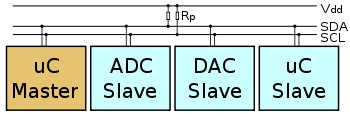
\includegraphics[width=0.3\columnwidth]{img/i2c-bus.png}
% 	\caption{Bus \IIC}%
% 	\label{fig:iic-bus}
% \end{wrapfigure}

